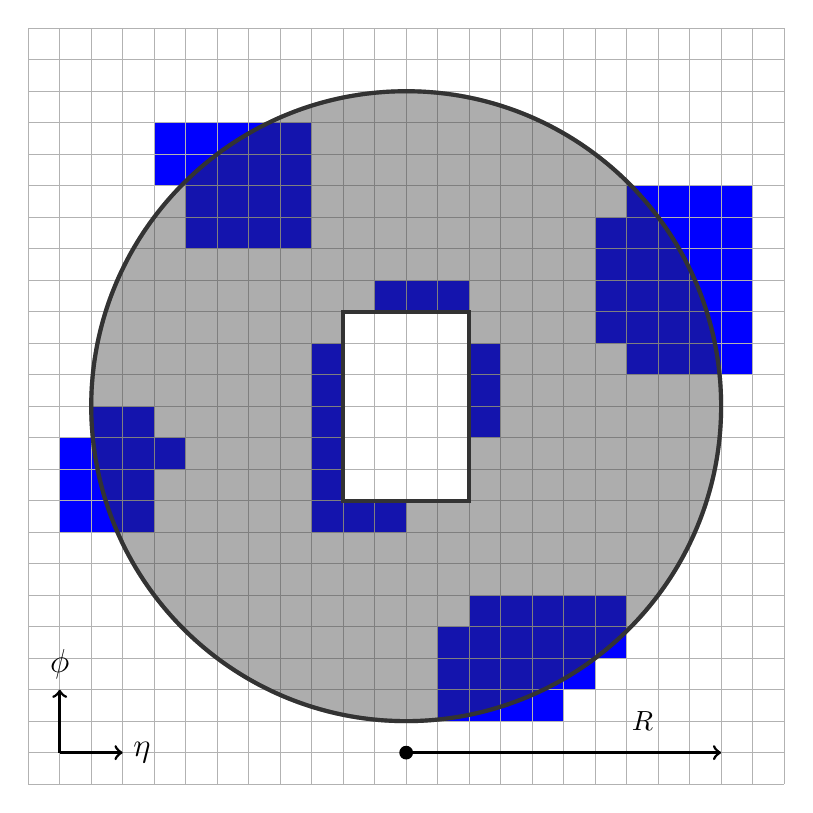
\begin{tikzpicture}

  %% middle
  \draw[blue,fill] (-1.2, -0.4) rectangle (1.2,0.4);
  \draw[blue,fill] (-0.8, -0.8) rectangle (0.8,0.0);
  \draw[blue,fill] (-1.2, 0.4) rectangle (1.2,0.8);
  \draw[blue,fill] (-0.4, -0.8) rectangle (0.4,-1.2);
  \draw[blue,fill] (-0.4, 0.8) rectangle (0.8,1.6);
  \draw[blue,fill] (-1.2, -0.0) rectangle (-0.0,-1.6);

  %% izq arriba
  \draw[blue,fill] (-1.2, 2) rectangle (-2.8,3.6);
  \draw[blue,fill] (-2.8, 3.2) rectangle (-3.2, 3.6);
  \draw[blue,fill] (-2.8, 2.8) rectangle (-3.2, 3.2);

  %% izq abajo
  \draw[blue,fill] (-3.2, -0.4) rectangle (-4.4,-1.6);
  \draw[blue,fill] (-2.8, -0.4) rectangle (-3.2,-0.8);
  \draw[blue,fill] (-3.2, -0.0) rectangle (-4.0,-0.4);

  %% der arriba
  \draw[blue,fill] (2.8, 0.4) rectangle (4.4,2.8);
  \draw[blue,fill] (2.4, 0.8) rectangle (2.8,2.4);

  %% der abajo
  \draw[blue,fill] (0.4, -2.8) rectangle (2.0,-4.0);
  \draw[blue,fill] (0.8, -2.4) rectangle (2.0,-2.8);
  \draw[blue,fill] (2.0, -2.4) rectangle (2.4,-3.6);
  \draw[blue,fill] (2.4, -2.4) rectangle (2.8,-3.2);

  % grid/cone
  \draw[step=0.4,black!30,thin] (-4.8,-4.8) grid (4.8,4.8);

  \draw[black!80, line width=1.5] (0,0) circle (4);
  \draw[black!80, line width=1.5, fill, opacity=0.4] (0,0) circle (4);

  \draw[black!80, line width=1.5, fill=white] (-0.8,-1.2) rectangle (0.8,1.2);
  \draw[step=0.4,black!30,thin] (-0.8,-1.2) grid (0.8,1.2);
  \draw[black!80, line width=1.5] (-0.8,-1.2) rectangle (0.8,1.2);


  \draw[->, line width=1] (-4.4,-4.4) -- (-3.6,-4.4) node[right] {\large $\eta$};
  \draw[->, line width=1] (-4.4,-4.4) -- (-4.4,-3.6) node[above] {\large $\phi$};

  \draw[->, line width=1] (0, -4.4) -- (4, -4.4);
  \draw[fill] (0, -4.4) circle(0.08);

  \node at (3,-4) {$R$};

 % \draw[dashed, line width=1] (0,0) -- (0,4);
%  \draw[fill] (0,0) circle(0.08);
%  \draw[fill] (0,4) circle(0.08);
 % \node at (0.5,2.5) (R) {\large $R$};
  %\node at (0,2) (mid) {};

  %% \draw[->] (mid) edge[bend right] (R);

\end{tikzpicture}
